% Vorlesung vom 07.01.2016
\renewcommand{\ldate}{2016-01-07}
%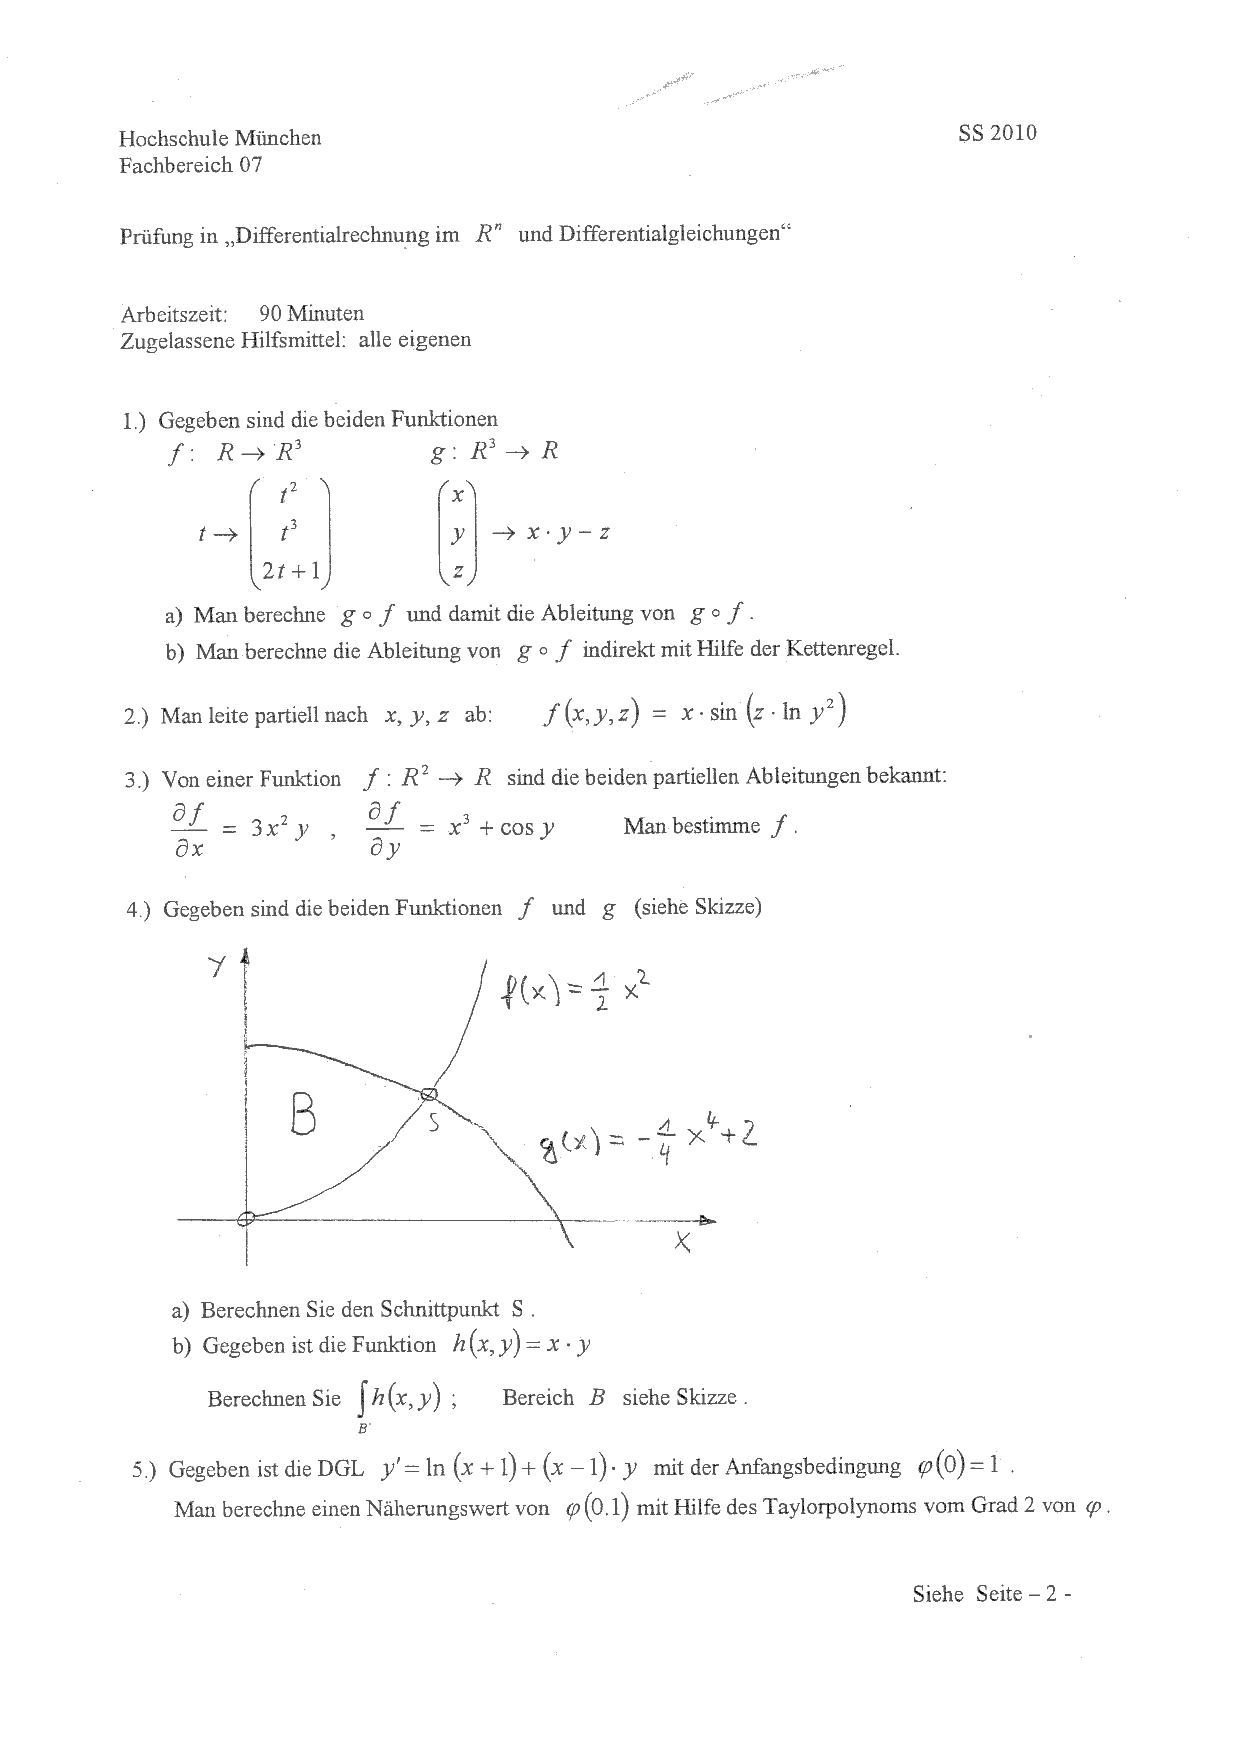
\includepdf[pages=-]{pruefungsangabe_diff_ss2010}

\section{Lösung für die Prüfung SS 2010}

\subsection{zu 1a)}
$ g\circ f) (t) = g\vektor{t^2\\t^2\\2t+1} = t^2 t^3 - (2t+1) = t^5 - 2t - 1$

$ (g\circ f)' (t) = 5 t^4 - 2$

\subsection{zu 1b)}
$ f'(t) = \vektor{2t\\3 t^2\\2}, g'\vektor{x\\y\\z} = \rbr{\frac{\delta g}{\dx},\frac{\delta g}{\dy},\frac{\delta g}{\dz}} = \rbr{y,x,-1} $

$g'(f(t)) \cdot f'(t) = g' \vektor{t^2\\t^3\\2t+1} \cdot \vektor{2t\\3t^2\\2} = \rbr{t^3, t^2, -1} \cdot \vektor{2t\\3t^2\\2} = 2t^4 \cdot 3t^4 - 2 = 5t^4 - 2 \checkmark$

\subsection{zu 2)}
$ f(x,y,z) = x\cdot \sin (z\cdot \ln y^2) = x \cdot \sin (2z \ln y)$

$ \frac{\df}{\dx} = \sin(z\cdot 2 \ln y)$

$\frac{\df}{\dy} = x\cdot \cos (z\cdot 2 \ln y) \cdot 2z \cdot \frac{1}{y} $

$\frac{\df}{\dz} = x\cdot \cos (z\cdot 2 \ln y) \cdot 2 \ln y$

\subsection{zu 3)}
Zum ersten Ausdruck: 
$ f(x,y) = 3y \cdot \frac{1}{3} x^3 + h(y) = yx^3 + h(y) $

Zum zweiten Ausdruck: 
$ f(x,y) = x^3 y + \sin y + g(x) $

$\Rightarrow h(y) = \sin y + g(x)$ In g(x) darf kein x vorkommen, also muss es eine Konstante sein: 
$ h(y) = \sin y + c$

$ f(x,y) = x^3y + \sin y + c $

\subsection{zu 4a)}
$ f(x) = g(x) $\\
$ \frac{1}{2} x^2 = -\frac{1}{4} x^4 + 2$ mit $x^2 = z$\\
$ \frac{1}{2} z = -\frac{1}{4} z^2 + 2 $\\
$ \Rightarrow z_1 = 2, z_2 = -4$\\
$z_2$ ist nicht möglich. $\Rightarrow z=2, x^2 = 2, x=\pm \sqrt{2} \Rightarrow x=\sqrt{2}$

\subsection{zu 4b)}
$ h(x,y) = x\cdot y$

$ \int_{B} h(x,y) 
= \int_{0}^{\sqrt{2}} \rbr{\int_{f(x)}^{g(x)} x \cdot y} dx 
= \int_{0}^{\sqrt{2}} \rbr{\sbr{\frac{1}{2} xy^2}_{y=f(x)}^{y=g(x)}} dx 
= \int_{0}^{\sqrt{2}} \frac{1}{2} x \sbr{\rbr{-\frac{1}{4} x^4 + 2}^2 - \rbr{\frac{1}{2} x^2}^2} dx 
= \int_{0}^{\sqrt{2}} \frac{1}{2} x \sbr{\frac{1}{16} x^8 + 4 - x^4 - \frac{1}{4} x^4} dx
= \frac{1}{2} \int_{0}^{\sqrt{2}} \rbr{\frac{1}{16} x^9 - \frac{5}{4} x^5 + 4x} dx
= \frac{1}{2} \sbr{\frac{1}{16} \cdot \frac{1}{10} x^{10} - \frac{5}{4} \cdot \frac{1}{6} x^6 + 4 \cdot \frac{1}{2} x^2}_0^{\sqrt{2}}
= 1.27
$

\subsection{zu 5)}
$ y' = \ln (x+1) + (x-1)\cdot y$ mit $ \varphi(0) = 1 $

Taylorpolynom: $\varphi(x) \approx \varphi(0) + \varphi'(0) \cdot x + \frac{\varphi''(0)}{2!} \cdot x^2$

$\varphi(0) = 1$

$\varphi'(0) = \ln(0+1) + (0-1) \cdot \varphi(0) = \ln 1 - 1 = -1$

$\varphi'(x) = \ln(x+1) + (x-1) \cdot \varphi(x)$

$\varphi''(x) = \frac{1}{x+1} + 1 \cdot \varphi(x) + (x-1)\cdot \varphi'(x)$

$ \varphi''(0) = 1 + 1 \cdot 1 - 1 \cdot - 1 = 3$

$\Rightarrow \varphi(x) \approx 1 - x + \frac{3}{2} x^2 $

$ \varphi(0.1) \approx 1 - 0.1 + \frac{3}{2} \cdot 0.01 = 0.915 $

\subsection{zu 6)}
P im u, v Koordinatensystem: 

u Wert: $\rbr{\cos \psi} + 2$ \profnote{Daheim nochmal anschauen}

v Wert: $ - \sin \psi$

$\psi$ ist die Bogenlänge (Der fette Bogen beim kleinen Kreis!).

$\psi = R \cdot \varphi = 3 \varphi$

$(u,v) = (2 + \cos \psi, -\sin \psi)$

Drehung um den Winkel $\varphi$: 

Drehmatrix: $\vektor{\cos \varphi, -\sin \varphi\\\sin \varphi, \cos \varphi}$

Koordinaten von P im xy-System:
 
$ \vektor{\cos \varphi, -\sin \varphi\\\sin \varphi, \cos \varphi} \vektor{2 + \cos 3 \varphi\\-\sin 3\varphi}
= \vektor{2\cos \varphi + \cos \varphi \cos 3 \varphi + \sin \varphi \sin 3 \varphi\\2\sin \varphi + \sin \varphi \cos 3 \varphi - \cos \varphi \sin 3 \varphi}
$

